\section{Planning}
\label{sec:orga82318d}
In fig. \ref{fig:gantt-diag2} is illustrated the Gantt diagram for the project and in
fig. \ref{fig:gantt-tasks} the tasks' descriptions. It should be noted that the project
tasks of Analysis, Design, Implementation and Tests are performed in two
distinct iterations as corresponding to the Waterfall project methodology. The
tasks are described as follows:
\begin{itemize}
\item \uline{Project Kick-off}: in the project lift-off, the group is formed and the tutor
is chosen. A brainstorming about conceivable devices takes place, whose
viability is then assessed, resulting in the product concept definition
(Milestone 0).
\item \uline{State of the Art}: in this stage, the working principle of the device is
studied based on similar products and the system components and its
characteristics are identified.
\item \uline{Analysis}: In the first stage --- Analysis 1 --- contains the analysis
results of the state of the art. It should yield the specifications document,
containing the requisites and restrictions to the project/product, on a
quantifiable basis as required to initiate the design; for example, the
car maximum velocity must be, at maximum, \texttt{2 m/s}. The second stage --- Analysis 2
--- contains the analysis of the first iteration of the development cycle.
\item \uline{Design}: it is done in two segments: modules design --- where the modules are
designed; integration design --- where the interconnections between modules is
designed. It can be subdivided into \emph{conceptual design} and \emph{solution
design}. 
\begin{itemize}
\item In the conceptual design, several problem solutions are identified,
quantifying its relevance for the project through a measuring scale,
inserted into an evaluation matrix, for example, Quality Function Deployment
(QFD).
\item In the solution design, the selected solution is developed. It must include
the solution modelling, e.g.:
\begin{itemize}
\item Control system design: analytically and using simulation
\item Transducer design: circuit design and simulation
\item Power system design: power supply, motors actuation and respective
circuitry design and simulation
\item Software design: for all required modules, and considering its
interconnections.
\end{itemize}
\end{itemize}
\item \uline{Implementation}: product implementation which is done by \uline{modules} and
\uline{integrated}. In the first stage, the implementation is done in a prototyping
environment using breadboards, yielding prototype alpha; in the second stage
it must include the veroboards or Printed Circuit Boards (PCBs), yielding
prototype beta.
\item \uline{Tests}: unit tests --- \uline{by modules} --- and integrated tests are
performed. Tests are considered as those performed over any physical
component or prototype. It contains all the tests conducted into the system
and the several prototypes.
\item \uline{Verification/Validation}: after the alpha prototype is built the
specifications listed in the analysis must be verified and the prototype
validated by an external agent (an external user to the group).
\item \uline{Delivery}: --- project closure encompassing:
\begin{enumerate}
\item Final prototype built, verified and validated.
\item Support documentation: how to replicate, instruction manual.
\item Final report: \textit{<2020-06-18 Thu>}
\item Public presentation: \textit{<2020-06-19 Fri> }
\end{enumerate}
\end{itemize}

\begin{figure}[htbp]
\centering
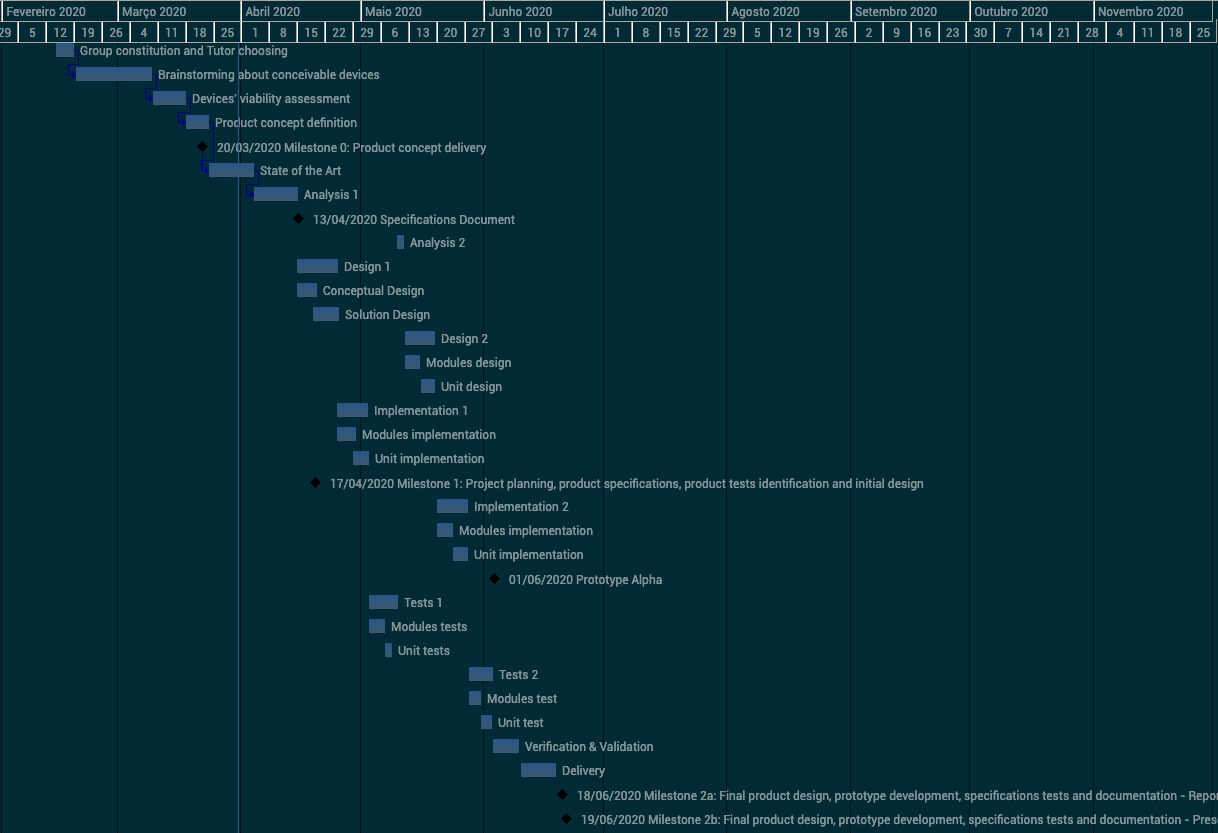
\includegraphics[width=1.0\textwidth]{./sec/img/gantt-diag-orig.png}
\caption{\label{fig:gantt-diag2}Project planning: Gantt diagram 1}
\end{figure}
\begin{figure}[htbp]
\centering
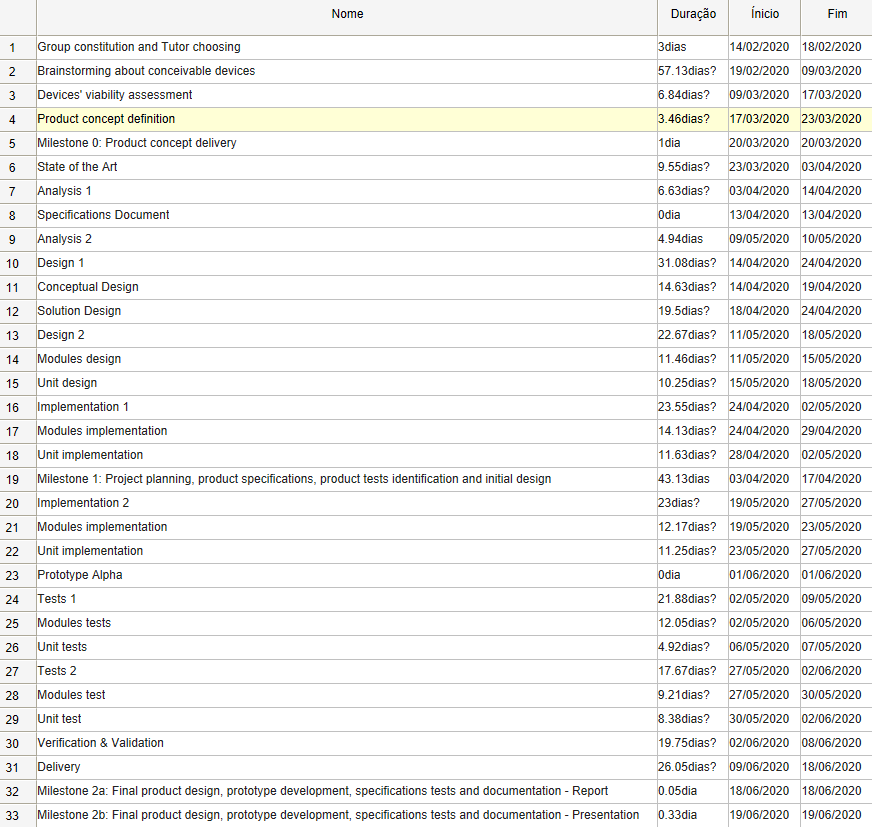
\includegraphics[width=1.0\textwidth]{./sec/img/gantt-orig-tasks.png}
\caption{\label{fig:gantt-tasks}Project planning: tasks}
\end{figure}
%%% Local Variables:
%%% mode: latex
%%% TeX-master: "../Phase1"
%%% End:
